\acresetall
Applications

\section{Chronic remapping}\label{sec:applications:chronic}
chronic remapping

\section[Gating of hippocampal activity, plasticity, and memory by entorhinal cortex long-range inhibition]{Gating of hippocampal activity, plasticity, and memory by entorhinal cortex long-range inhibition\footnote{This work has been previously published \citep{Basu2016} and is joint work with the coauthors.}}
LRIP
\begin{quote}
The cortico-hippocampal circuit is critical for storage of associational memories. Most studies have focused on the role in memory storage of the excitatory projections from entorhinal cortex to hippocampus. However, entorhinal cortex also sends inhibitory projections,whose role in memory storage and cortico-hippocampal activity remains largely unexplored. We found that these long-range inhibitory projections enhance the specificity of contextual and object memory encoding. At the circuit level, these g-aminobutyric acid (GABA)–releasing projections target hippocampal inhibitory neurons and thus act as a disinhibitory gate that transiently promotes the excitation of hippocampal CA1 pyramidal neurons by suppressing feedforward inhibition. This enhances the ability of CA1 pyramidal neurons to fire synaptically evoked dendritic spikes and to generate a temporally precise form of heterosynaptic plasticity. Long-range inhibition from entorhinal cortex may thus increase the precision of hippocampal-based long-term memory associations by assessing the salience of mnemonic information to the immediate sensory input.
\attrib{\citealt{Basu2016}}
\end{quote}

\begin{figure}
	\centering
	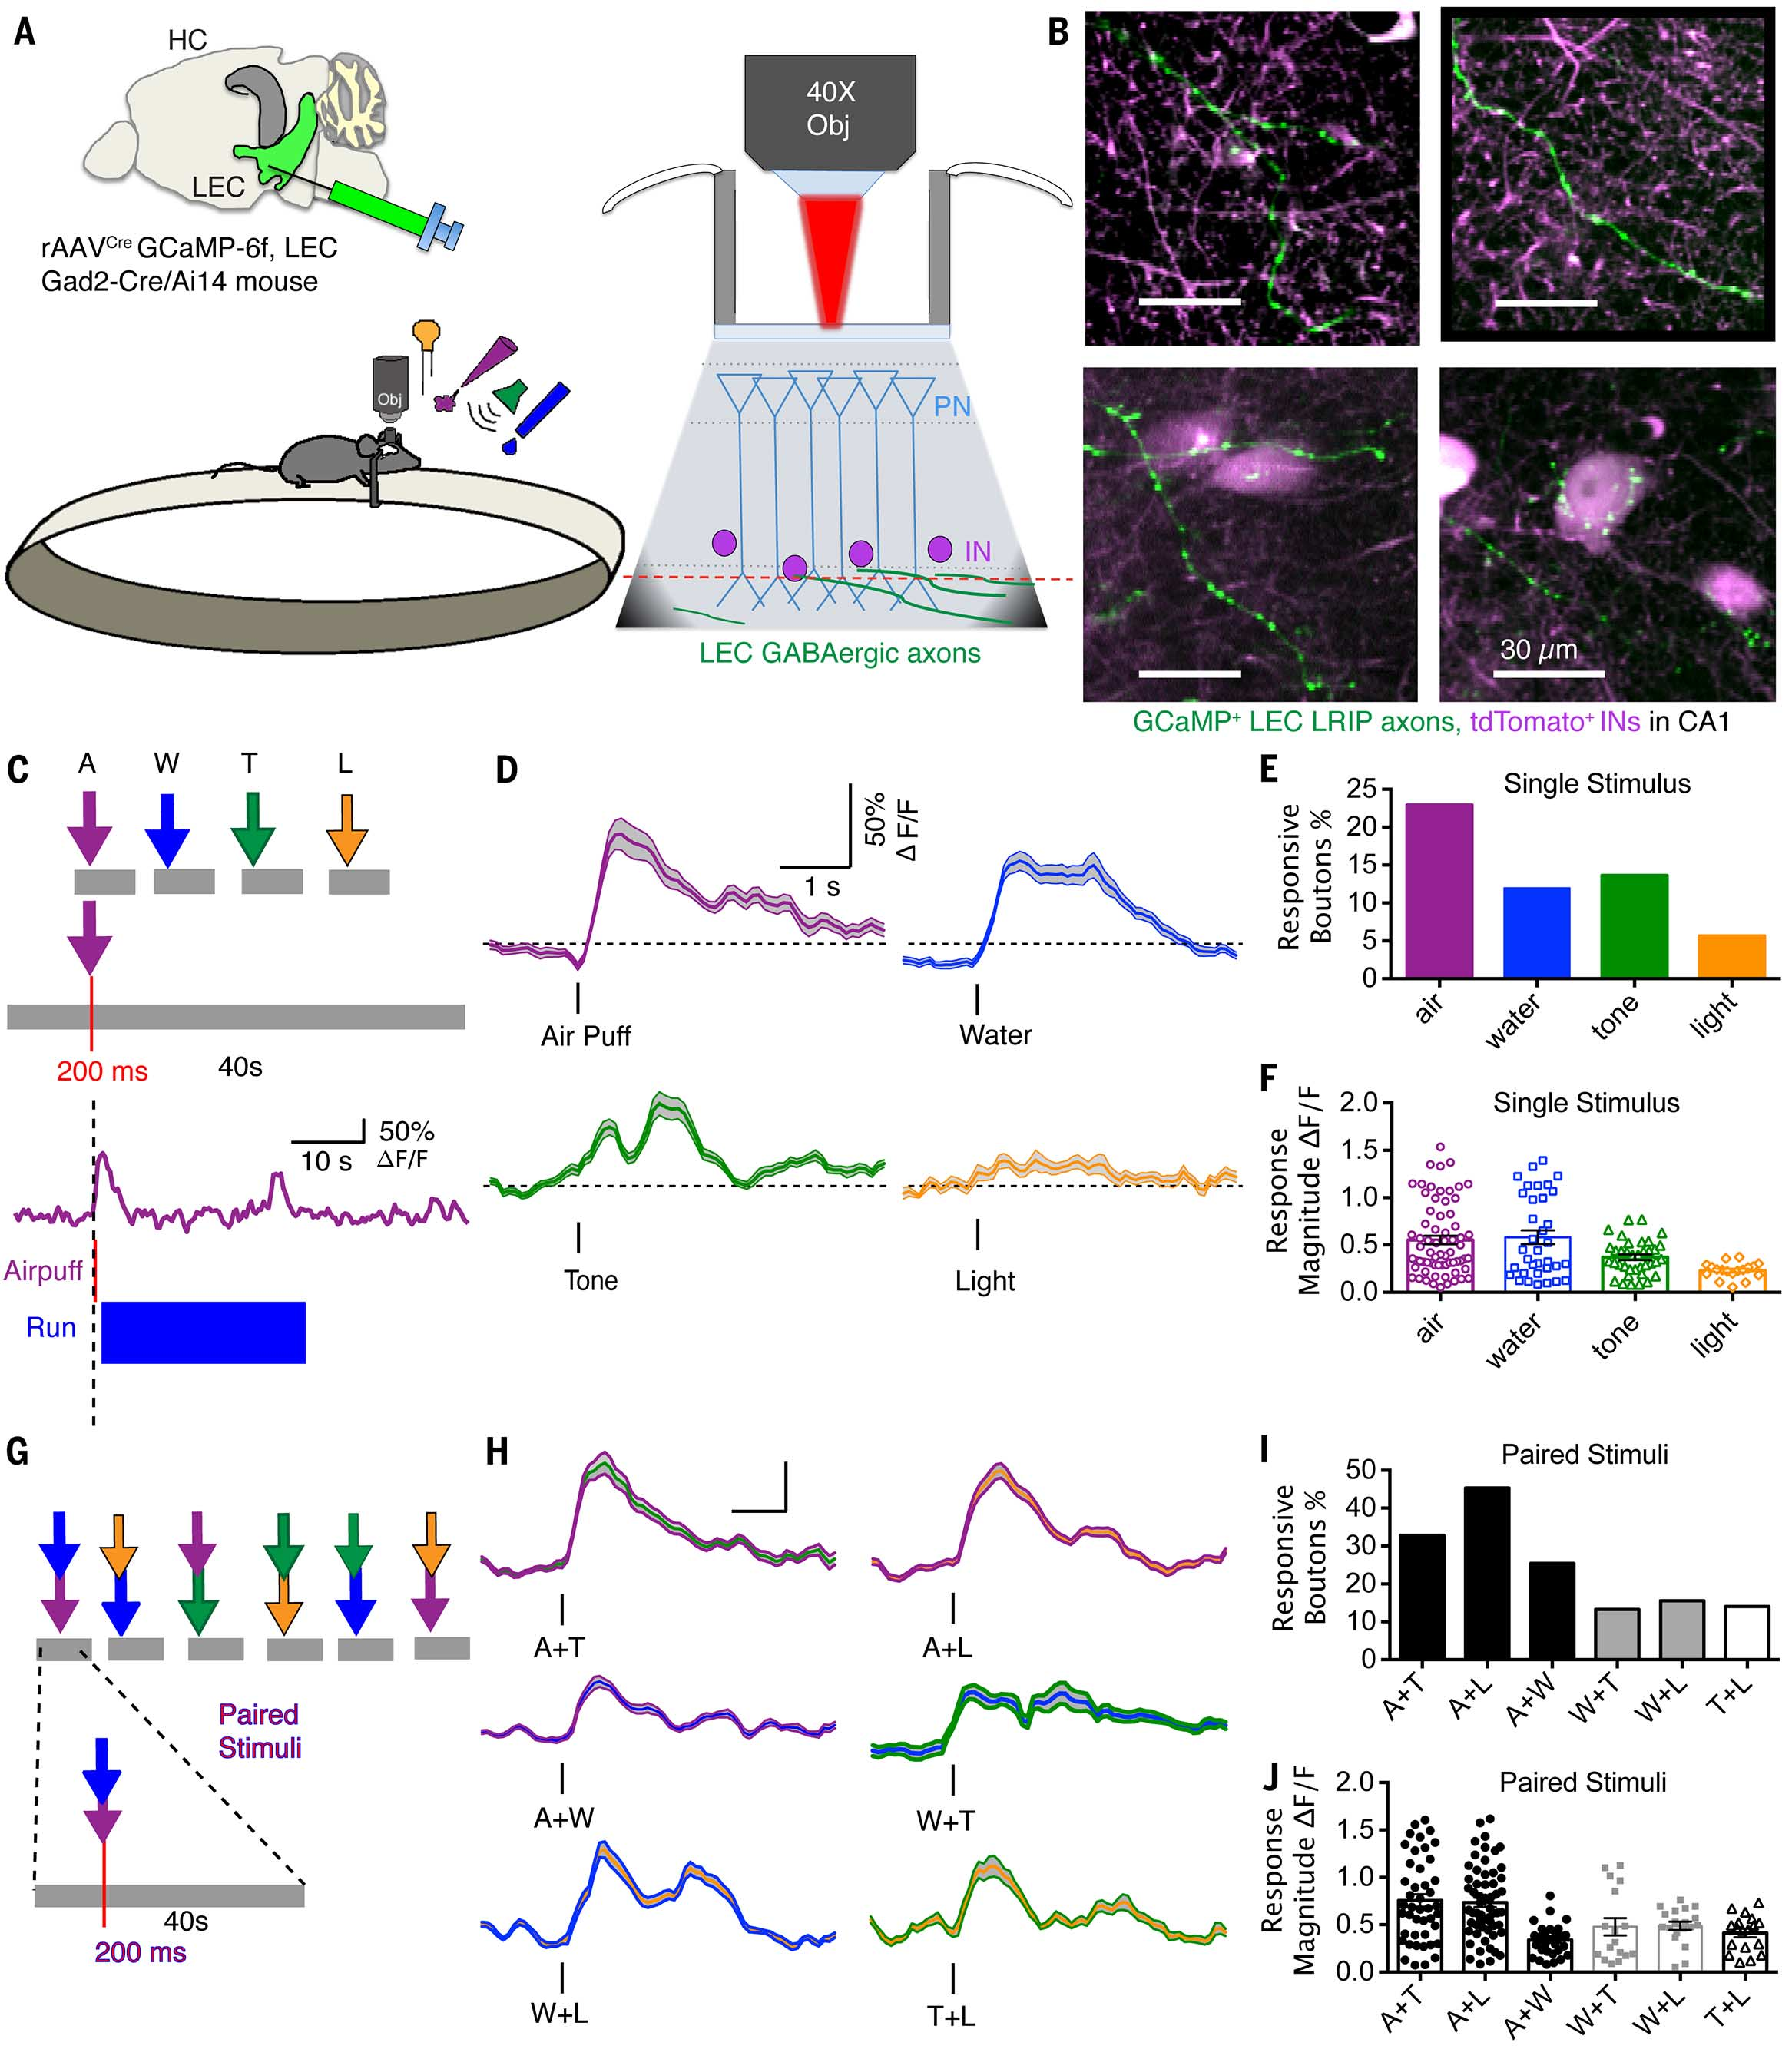
\includegraphics[width=0.75\textwidth]{applications/LRIP_Fig3}
	\caption[Functional imaging of sensory coding in LEC LRIPs present in SLM of CA1]{Functional imaging of sensory coding in LEC LRIPs present in SLM of CA1.
	A) Diagram of in vivo imaging experiment. GCaMP6f was expressed in dorsal LEC, by injecting Cre-dependent rAAV in \emph{Gad2-Cre/Ai} 14 mice that also expressed tdTomato in all GABAergic neurons. A 40x water immersion objective was used for two-photon imaging through a cranial window over CA1 in head-fixed awake mice during multimodal sensory and behavioral stimuli presentation.
	(B) Four examples of time-averaged images of GCaMP6f fluorescence in LEC LRIP axons in SLM (green) with tdTomato labeling CA1 interneurons (magenta).
	(C) Experimental design of single-stimulus protocol. Imaging was performed in blocks of four trials, each 40 seconds in duration. After a 10~$\pm$~3~s baseline, one of four types of stimuli -- aversive air puff (A), water drop (W), tone (T), or light (L) -- was presented in random order for 200~ms, except the water drop was limited to 50~ms to prevent satiation. Each block was repeated to obtain at least five trials per stimulus. The animal's behavioral response (running and licking) was monitored. $\Delta F/F$ traces showing increased Ca\super{2+} signal in a single bouton on an LRIP axon in response to air puff.
	(D) Mean ($\pm$ SEM) $\Delta F/F$ Ca\super{2+} signal (PSTH) from responsive ROIs to indicated stimuli.
	(E) Percentage of responsive boutons to the stimuli (air = 22.92\%, water = 11.96\%, tone = 13.64\%, and light = 5.65\%).
	(F) Scatter and mean ($\pm$ SEM) plots of $\Delta F/F$ signals from individual responsive boutons (air = 0.55~$\pm$~0.05, n = 68; water = 0.58~$\pm$~0.07, n = 35; tone = 0.37~$\pm$~0.03, n = 37; light = 0.23~$\pm$~0.02, n = 18).
	(G) Experimental protocol: Imaging was performed as described above, but in response to pairs of stimuli, presented in blocks of 10 trials, each 40 seconds long. Stimuli were randomized and paired stimuli were interleaved with single stimulus presentations.
	(H) Mean ($\pm$ SEM) $\Delta F/F$ Ca\super{2+} signal (PSTH) from responsive ROIs to paired stimuli.
	(I) Percentage of responsive boutons for paired stimuli (A+T = 32.8\%; A+L = 45.3\%; A+W = 25.4\%; W+T = 13.3\%; W+L = 15.6\%; T+L = 14.1\%).
	(J) Scatter and mean ($\pm$ SEM) plots of $\Delta F/F$ signals to paired stimuli from individual responsive boutons (A+T = 0.76~$\pm$~0.07, n = 44; A+L = 0.74~$\pm$~0.05, n = 58; A+W = 0.34~$\pm$~0.03, n = 31; W+T = 0.48~$\pm$~0.09, n = 17; W+L = 0.49~$\pm$~0.04; T+L = 0.41~$\pm$~0.045, n = 18).}
	\label{fig:applications:LRIP:imaging}
\end{figure}

\section[Distinct Contribution of Adult-Born Hippocampal Granule Cells to Context Encoding]{Distinct Contribution of Adult-Born Hippocampal Granule Cells to Context Encoding\footnote{This work has been previously published \citep{Danielson2016a} and is joint work with the coauthors.}}

While this project is the primary work of the first author, the behavioral apparatus, experimental paradigms, and analysis tools were all developed jointly.
In particular, this manuscript was Attila Losonczy's lab's first publication of head-fixed two-photon calcium imaging of place cells in mice, so replied upon upgrades to the behavioral aparatus (\autoref{sec:intro:techniques:behavior}), the imaging processing pipeline (\autoref{sec:intro:techniques:pipeline}), and analysis of place cell data (\autoref{sec:intro:techniques:place-cells}).

% In brief, dentate gyrus granule cells are one of the few populations of neurons that undergoes continue neurogenesis in the adult mammalian brain.
\begin{quote}
Adult-born granule cells (abGCs) have been implicated in cognition and mood; however, it remains unknown how these cells behave in vivo. Here, we have used two-photon calcium imaging to monitor the activity of young abGCs in awake behaving mice. We find that young adult-born neurons fire at a higher rate in vivo but paradoxically exhibit less spatial tuning than their mature counterparts. When presented with different contexts, mature granule cells underwent robust remapping of their spatial representations, and the few spatially tuned adult-born cells remapped to a similar degree. We next used optogenetic silencing to confirm the direct involvement of abGCs in context encoding and discrimination, consistent with their proposed role in pattern separation. These results provide the first in vivo characterization of abGCs and reveal their participation in the encoding of novel information.
\attrib{\citealt{Danielson2016a}}
\end{quote}

\begin{figure}
	\centering
	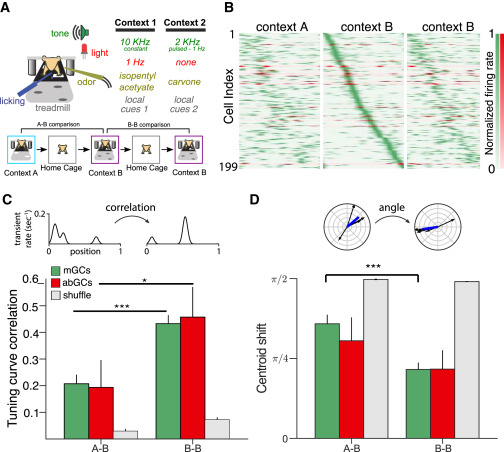
\includegraphics[width=0.8\textwidth]{applications/abGC_Fig3}
	\caption[Contextual coding by adult-born and mature granule cells]{Contextual coding by adult-born and mature granule cells.
	A) Experimental schematic. Mice ran for three 12-min sessions in contexts A, B, and B (1 hr between runs). A and B refer to either context 1 or 2 (chosen randomly for each experiment).
	(B) Remapping of spatial rate maps across sequential context exposures. Smoothed calcium transient rates, normalized to peak for each cell, are plotted as a function of position during three contextual exposures (A, B, B). Cells (mGCs, green; abGCs, red) are ordered according to the position of peak activity during the first exposure to context B. Data is shown for GCs with sufficient tuning specificity and activity (p~$<$~0.1, at least four transients) in at least one experiment.
	(C and D) Context specificity of spatial representations. Tuning curve correlations of 1D rate maps (C) and centroid shifts (angle between tuning directions) (D) between sequential exposures to different (A-B) or the same (B-B) contexts for all cells shown in (B) (A-B: n~=~180 mGCs, 14~abGCs; B-B: n~=~174 mGCs, 9~abGCs). The rate map correlations of both populations were more similar in the B-B condition than in A-B (Mann-Whitney U, mGCs: U(150)~=~5,291, p~$<$~0.001; abGCs: U(18)~=~23.0, p~$<$~0.05). In mGCs the tuning shift was larger in the A-B condition than in B-B, although this did not reach significance in abGCs (mGCs: U(150) = 5,714, p~$<$~0.001; abGCs: U(18)~=~40.0, p~=~0.34). In both conditions, the similarity of spatial representations exceeded chance levels as estimated by shuffling cell identity (gray).
	Error bars are mean~$\pm$~SEM.}
	\label{fig:applications:dg:context}
\end{figure}

\section[Sublayer-Specific Coding Dynamics during Spatial Navigation and Learning in Hippocampal Area CA1]{Sublayer-Specific Coding Dynamics during Spatial Navigation and Learning in Hippocampal Area CA1\footnote{This work has been previously published \citep{Danielson2016b} and is joint work with the coauthors.}}

\begin{quote}
The mammalian hippocampus is critical for spatial information processing and episodic memory. Its pri- mary output cells, CA1 pyramidal cells (CA1 PCs), vary in genetics, morphology, connectivity, and elec- trophysiological properties. It is therefore possible that distinct CA1 PC subpopulations encode different features of the environment and differen- tially contribute to learning. To test this hypothesis, we optically monitored activity in deep and superfi- cial CA1 PCs segregated along the radial axis of the mouse hippocampus and assessed the relationship between sublayer dynamics and learning. Superficial placemapswere more stable than deep during head- fixed exploration. Deep maps, however, were prefer- entially stabilized during goal-oriented learning, and representation of the reward zone by deep cells predicted task performance. These findings demon- strate that superficial CA1 PCs provide a more stable map of an environment, while their counterparts in the deep sublayer provide a more flexible represen- tation that is shaped by learning about salient fea- tures in the environment.
\attrib{\citealt{Danielson2016b}}
\end{quote}